\documentclass[12pt]{article}

\usepackage{sbc-template}
\usepackage{graphicx,url}

\usepackage[T1]{fontenc} 
\usepackage[brazilian]{babel}   
\usepackage[utf8]{inputenc}
\usepackage{enumitem}
\usepackage{placeins}
\usepackage{float}

\hyphenation{english terms to not hyphenize various non repeatable words here something like long word Portuguese}
     
\sloppy


\title{Relatório de Programação Concorrente e Distribuida}

\author{Ana L. Tomita\inst{1}, Fabricio M. Muller\inst{1}, Gabriel A. Garcia\inst{1}, \\Gabriel V. F. do Carmo\inst{1}, Loren P. R. Lorenzetto\inst{1}. }

\address{Instituto de Ciência e Tecnologia -- Universidade Federal de São Paulo
  (Unifesp)
  \email{\{%
    gabriel.almeida12,%
    rafael.lorenzetto,%
    gabriel.fabri,%
    tomita.ana,%
    fmmuller%
    }
    \email{
    \}@unifesp.br}
}

\begin{document} 


\maketitle
     
\begin{resumo} 
  A multiplicação de matrizes é uma operação fundamental em diversas áreas da computação e, em sua forma clássica, possui custo $O(n^3)$, o que a torna adequada para técnicas de paralelização e de otimização do acesso à memória. Este trabalho implementa e compara duas abordagens paralelas com OpenMP: uma implementação em blocos, baseada em divisão e conquista com vetorização SIMD e comparada à biblioteca OpenBLAS, e o algoritmo de Strassen, que reduz a complexidade assintótica para $O(n^{\log_{2}7})$. O desempenho foi avaliado por meio do tempo de execução, do \textit{overhead} paralelo total, do \textit{speedup} e da eficiência, variando o tamanho das matrizes e o número de \textit{threads}. Na implementação em blocos, com 16 \textit{threads}, o parâmetro de corte $k_c$ mostrou-se determinante: blocos pequenos resultaram em desempenho reduzido, enquanto blocos maiores alcançaram \textit{speedup} de até 8.66x e eficiência de 54.10\% em matrizes \textit{double} de 4000x4000. No método de Strassen, o uso de 8 \textit{threads} apresentou o melhor equilíbrio entre \textit{speedup} e eficiência, e o \textit{speedup} com 16 \textit{threads} superou 7x em matrizes de 300x300.
\end{resumo}


\section{Introdução}

O desempenho dos processadores crescia cerca de 52\% ao ano até 2002 \cite{herlihy2008}, mas desde então esse ritmo desacelerou devido ao limite físico do silício \cite{hennessy2017}. Por volta de 2005, a maioria dos fabricantes passou a apostar na programação paralela como caminho para novos ganhos de desempenho \cite{pacheco2011}, o que exige que o \textit{software} utilize múltiplos núcleos de maneira eficiente.

Nesse contexto, a multiplicação de matrizes é um problema interessante, por ser operação central em áreas como álgebra linear computacional, simulações científicas e aprendizado de máquina. Seu algoritmo clássico possui custo $O(n^3)$ \cite{cormen2012} e, como os elementos da matriz resultante podem ser calculados de forma independente, o problema é adequado a paralelismo de dados. Porém, o desempenho também depende do acesso à memória, sendo que a localidade espacial, o uso da \textit{cache} e a vetorização têm papel decisivo \cite{hennessy2017, allen2002}. Por outro lado, algoritmos como o de Strassen reduzem a complexidade assintótica para $O(n^{\log_{2}7})$ \cite{ikenmeyer2019strassen} e, por dividirem o problema em 7 multiplicações independentes, também contém oportunidades de paralelização, desde que a criação de tarefas seja controlada para que o custo incorrido não supere o ganho obtido.

O objetivo deste trabalho é implementar e comparar duas abordagens paralelas para a multiplicação de matrizes: uma implementação em blocos, que busca explorar a hierarquia de memória, e o algoritmo de Strassen, que reduz o número de multiplicações por meio de divisão e conquista. Ambas foram desenvolvidas em C/C++, paralelizadas com OpenMP e avaliadas por meio do tempo de execução, do \textit{overhead} paralelo total, do \textit{speedup} e da eficiência \cite{grama2003}, considerando diferentes tamanhos de matrizes e quantidades de \textit{threads}.


\section{Fundamentação Teórica} \label{sec:firstpage}
\subsection{Computação Paralela}
Do período de 1986 até 2002, o desempenho dos processadores aumentava cerca de 52\% a cada ano \cite{herlihy2008}. No entanto, desde 2002 o crescimento de desempenho das novas gerações de microprocessadores tem desacelerado cada vez mais, dado o limite físico do silício \cite{hennessy2017}. Desse modo, por volta de 2005, a grande maioria das fabricantes de microprocessadores decidiu que o caminho para o ganho de desempenho estava direcionado à programação paralela \cite{pacheco2011}.
\par
\cite{pacheco2011} aponta que na computação paralela "um programa é aquele no qual múltiplas tarefas cooperam intimamente para resolver um problema". Nesse sentido, operações matriciais representam um problema adequado para o paralelismo, pois o cálculo de elementos diferentes pode ser distribuído em diferentes unidades de execução.
% Se houver espaço
%\subsection{Threads e Paralelismo}
%O conceito de \textit{thread} pode ser definido como uma linha de execução de um processo \cite{tanenbaum2016}. Comumente, existem dois tipos de paralelismo, o paralelismo de dados e de tarefas. O paralelismo de dados está relacionado a distribuição de subconjuntos de um mesmo dado entre multíplos processadores. Já o paralelismo de tarefas envolve a distribuição de \textit{threads} entre os núcleos. \cite{silberschatz2018}. Nesse sentido, o problema clássico da  multiplicação de matrizes é explorado como um problema de paralelismo de dados, uma vez que diferentes elementos da matriz resultante podem ser calculados de maneira independente.

\subsection{Multiplicação de Matrizes}
De acordo com \cite{cormen2012}, o problema clássico para multiplicação de matrizes envolve duas matrizes dadas, A e B, e C uma nova matriz a ser calculada. A operação que define cada elemento $C_{ij}$ pode ser dada como:
\begin{equation}
C_{ij} = \sum_{k=1}^{n} A_{ik}B_{kj}
\end{equation}
\par
Ou seja, cada elemento $C_{ij}$ é obtido pelo produto escalar entre a linha $i$
de A e a coluna $j$ de B. Dessa forma, o algoritmo sequencial possui um custo $O(n^3)$ para matrizes de dimensão N por N. 
\subsection{Vetorização}
Segundo \cite{allen2002} vetorização foi uma das técnicas que permitiram com que resultados ideais em diversas arquiteturas paralelas ocorressem em multiplicação de matrizes. A vetorização é uma técnica que permite explorar o paralelismo a nível de dados por meio de instruções SIMD (\textit{Single Instruction, Multiple Data}), ou seja, operação de múltiplos dados sobre a mesma instrução \cite{hennessy2017}. 
\par
Na vetorização automática o compilador identifica trechos específicos do código como laços de repetição, em que as operações podem ser realizadas de forma paralela em nível de instrução, e os transformam em instruções vetoriais compatíveis com os recursos do processador. Dessa forma, pode-se reduzir o número de instruções para processar um conjunto de dados, melhorando o tempo de execução de programas, permitindo que a multiplicação de matrizes seja executada em tempo ideal \cite{intel2023vectorization}. 

\subsection{Princípio da localidade espacial}
\cite{hennessy2017} mostram que segundo o princípio da localidade espacial, quando um dado é acessado, existe uma grande possibilidade de dados armazenados próximos serem necessários. Dessa forma, quando um dado não é encontrado em \textit{cache}, o processador busca um bloco de dados próximos ao dado na memória principal.
\par
Nesse sentido, segundo \cite{cppreference_array}, em C/C++ as matrizes multidimensionais são armazenadas em ordem \textit{row-major}, ou seja, elementos de uma mesma linha ocupam posições consecutivas na memória. Por conseguinte, percorrer os elementos de uma linha de forma consecutiva tende a favorecer a localidade espacial, já percorrer por coluna desfavorece o aproveitamento de dados em \textit{cache}.
\subsection{Transposição de matrizes}
\par
No cenário de multiplicação de matrizes o acesso à memória da matriz B terá um custo maior que A. Assim, a transposição da matriz, definido por \cite{cormen2012} como a permutação dos elementos de cada i-ésima linha, pela j-ésima coluna, pode resolver o problema do armazenamento na memória alterando apenas a forma de cálculo da matriz C para manter o resultado, computando com os elementos da linha "$j$" ao invés da coluna. 

\subsection{Algoritmo de Strassen para multiplicação de matrizes}
Segundo \cite{ikenmeyer2019strassen} o algoritmo de Strassen para multiplicação de matrizes foi uma descoberta revolucionária na álgebra linear computacional. A ideia central desse algoritmo é multiplicar matrizes de tamanho 2X2 com apenas 7 operações, utilizando a estratégia de divisão e conquista aplicar a matrizes N x N. O algoritmo surge da decomposição da forma: 
\begin{equation}
XY = \sum_{k=1}^{7} u_{k}(X)v_{k}(Y)W_{k}
\end{equation}
\par
Em que $u_k$ e $v_k$ são formas lineares escolhidas no espaço das matrizes 2X2 e $W_k$ são 7 matrizes de tamanho 2X2. Aplicando esse algoritmo é possível reduzir o custo computacional para $O(n^{\log_{2}7})$ operações aritméticas \cite{ikenmeyer2019strassen}.

\subsection{Métricas de Desempenho}
 Entre as principais métricas para avaliação do desempenho de algoritmos destacam-se: Tempo de execução; \textit{Overhead} paralelo total; \textit{Speedup}; Eficiência;
\par
\cite{grama2003} definem o tempo de execução de um algoritmo sequencial $T_s$ como o tempo decorrido entre o início e o fim de sua execução em um computador sequencial. Já o tempo de execução de um algoritmo paralelo $T_p$ é definido como o tempo decorrido a partir do momento em que a computação paralela se inicia até o momento da execução do último elemento de processamento.
\par
Os custos computacionais adicionados devido à paralelização são encapsulados em uma expressão chamada \textit{overhead}, que pode ser definida como o tempo total gasto por todos elementos coletivamente, além do tempo necessário pelo algoritmo sequencial \cite{grama2003}. Dessa forma, sendo $p$ o número de \textit{threads} \textit{overhead} paralelo total pode ser calculado como:
\begin{equation}
T_o = pT_p - T_s
\end{equation}
\par
\textit{Speedup} é a medida que mostra o benefício relativo de programar paralelamente em relação ao programa sequencial \cite{grama2003}. Assim, o \textit{Speedup} do sistema pode ser calculado como a razão do tempo de execução sequencial pelo tempo em paralelo como na equação abaixo:  
\begin{equation}
S_p = \frac{T_s}{T_p}
\end{equation}
\par
Já a eficiência é uma medida da fração de tempo na qual um elemento de processamento está utilmente empregado \cite{grama2003}. A eficiência pode ser calculada como:
\begin{equation}
E_p = \frac{T_s}{pT_p}.
\end{equation}


\section{Trabalhos Relacionados}

\subsection{Parallel matrix transpose algorithms on distributed memory concurrent computers}
O trabalho de \cite{art1} propõe algoritmos para a transposição de matrizes em computadores de memória distribuída. Os processadores são organizados em uma grade bidimensional $P \times Q$ e a matriz é distribuída em blocos de forma cíclica (\textit{block cyclic data distribution}). Quando o máximo divisor comum (MDC) entre $P$ e $Q$ é 1, todos os processadores precisam realizar comunicação total entre si; quando é maior que 1, os processadores são divididos em grupos delimitados pelo MDC, e as transposições entre blocos de um mesmo grupo ocorrem simultaneamente, reduzindo o tempo de execução.
\par
A análise do artigo mostra que transpor o resultado de uma multiplicação de matrizes com esse procedimento aumenta pouco o tempo total, e que o algoritmo suporta grades não quadradas ($P \neq Q$) mantendo alta eficiência, superando algoritmos restritos a grades quadradas. 

\subsection{Anatomy of High-Performance Matrix Multiplication}
O trabalho de \cite{art2} trata de implementações otimizadas da multiplicação de matrizes (GEMM), com foco no gerenciamento eficiente da hierarquia de memória. Os autores observam que algoritmos tradicionais não consideram características reais do hardware, como o número finito de entradas do \textit{Translation Look-aside Buffer} (TLB) e a latência das memórias \textit{cache}. Para evitar esses gargalos, a GEMM é reestruturada em níveis: no mais alto, o painel de $A$ é dimensionado para caber no \textit{cache} L2 (ou L3) e no limite de entradas do TLB, e os blocos de $B$ são empacotados em \textit{buffers} contíguos para fluir pelo \textit{cache} L1; no \textit{micro-kernel}, o processamento ocorre em pequenas submatrizes, maximizando o uso de instruções vetoriais e o paralelismo em nível de instrução.
\par
O algoritmo é utilizado em bibliotecas de computação de alto desempenho, como OpenBLAS e Intel MKL. Porém, o procedimento é elaborado e possui \textit{overhead} significativo, e não é recomendável para operações simples.
\par
Embora o presente trabalho não reconstrua diretamente nenhum dos métodos descritos, ambos os artigos apresentam esquemas de particionamento e estratégias de gerenciamento de recursos que serviram de referência para o desenvolvimento do projeto.


\section{Implementação}
\subsection{Implementação em blocos}

\par A primeira abordagem implementada e avaliada foi o algoritmo de multiplicação de matrizes baseado na estratégia de divisão e conquista (\textit{Divide and Conquer}), estruturado de forma recursiva para o particionamento de submatrizes. A técnica foi selecionada por permitir uma divisão estruturada do problema, cujos casos base são resolvidos por meio de uma rotina paralela customizada que integra diretivas OpenMP e otimização vetorial SIMD.
\par O código foi desenvolvido na linguagem C++ para poder utilizar templates para os tipos de dados e emprega a biblioteca OpenMP para a paralelização. Como o particionamento recursivo pode introduzir um custo elevado de gerência de tarefas, implementou-se um parâmetro limiar de corte ($k_c$), garantindo que o paralelismo e a vetorização sejam aplicados de forma equilibrada somente quando as submatrizes atingem dimensões adequadas. Ademais, o framework de testes realiza comparações diretas de exatidão e desempenho com as rotinas altamente otimizadas da biblioteca OpenBLAS (\textit{cblas\_sgemm} para precisão simples e \textit{cblas\_dgemm} para precisão dupla).
\par Os testes foram conduzidos considerando diferentes dimensões de matrizes quadradas (1000x1000, 2000x2000, 3000x3000 e 4000x4000) e uma variação ampla de valores para o limiar $k_c$. As matrizes de teste são populadas com valores em ponto flutuante gerados aleatoriamente (nos tipos \textit{float} e \textit{double}), utilizando alinhamento de memória específico para favorecer o desempenho das instruções de hardware.
\par As métricas de desempenho coletadas e analisadas compreendem o tempo de execução sequencial ($T_1$), o tempo de execução paralelo ($T_P$), o \textit{speedup}, a eficiência paralela, o \textit{overhead} paralelo total e o rendimento computacional medido em GFLOPS, permitindo confrontar a solução desenvolvida com os padrões industriais do OpenBLAS.

\subsection{Método de Strassen}
\par A segunda implementação escolhida para os testes foi o algoritmo de Strassen para multiplicação de matrizes. Este foi escolhido por possuir propriedades que tornam sua paralelização um caso relevante. Como discutido antes na fundamentação, Strassen efetua multiplicações em matrizes 2x2 utilizando 7 operações. Dado que essas são independentes entre si, é possível paralelizar sua execução para comparar eficiência.
As métricas de desempenho utilizadas na implementação são as mesmas vistas anteriormente, tempo de execução tanto sequencial quando paralelo, \textit{overhead} paralelo total, \textit{speedup} e eficiência.
\par O código foi implementado em C e utiliza OpenMP para efetuar sua paralelização. \textit{Multithreading} é utilizado para realizar operações de soma e subtração de matrizes em Strassen. Porém, algumas restrições foram implementadas para que o custo de gerenciar todas as tarefas não supere o ganho do paralelismo. Como o método utiliza recursão, a criação desregulada de tarefas pode diminuir a eficiência do programa. Por conta disso uma restrição foi colocada para que novas tarefas sejam criadas somente quando a matriz sendo computada seja de um dado tamanho.
\par As matrizes utilizadas são geradas de maneira aleatória com dimensão N x N determinada em tempo de execução, cada elemento povoado com um valor aleatório do tipo \textit{int} com valor variando entre -1000 e 1000.


\section{Resultados}

\subsection{Implementação em blocos}

\small
\setlength{\tabcolsep}{3.5pt}
\begin{table}[H]
    \centering
    \caption{Resultados da implementação em blocos para matrizes de 1000x1000 e 2000x2000}
    \label{tab:Blocos1000_4000}
    \small
    \setlength{\tabcolsep}{3.5pt}
    \begin{tabular}{|c|l|c|c|c|c|c|c|c|}
        \hline
        \textbf{Matriz} & \textbf{Tipo} & \textbf{$k_c$} & \textbf{Tempo (s)} & \textbf{GFLOPS} & \textbf{$T_1$ (1 thd)} & \textbf{Overhead (s)} & \textbf{Speedup} & \textbf{Eficiência} \\ \hline
        \multicolumn{9}{|c|}{\textbf{Matriz 1000x1000 | Ref: cblas\_sgemm (0.0060s, 333.33 GFLOPS)}} \\ \hline
        1000x1000 & float & 64   & 2.3710 & 0.84 & 2.2750 & 35.6610 & 0.96 x & 6.00 \% \\ \hline
        1000x1000 & float & 96   & 2.4080 & 0.83 & 2.4100 & 36.1180 & 1.00 x & 6.26 \% \\ \hline
        1000x1000 & float & 128  & 0.7740 & 2.58 & 2.4180 & 9.9660  & 3.12 x & 19.53 \% \\ \hline
        1000x1000 & float & 192  & 0.5230 & 3.82 & 2.5550 & 5.8130  & 4.89 x & 30.53 \% \\ \hline
        1000x1000 & float & 256  & 0.4040 & 4.95 & 2.3990 & 4.0650  & 5.94 x & 37.11 \% \\ \hline
        1000x1000 & float & 384  & 0.4140 & 4.83 & 2.3220 & 4.3020  & 5.61 x & 35.05 \% \\ \hline
        1000x1000 & float & 512  & 0.3620 & 5.52 & 2.4250 & 3.3670  & 6.70 x & 41.87 \% \\ \hline
        1000x1000 & float & 1000 & 0.3270 & 6.12 & 2.2260 & 3.0060  & 6.81 x & 42.55 \% \\ \hline
        \multicolumn{9}{|c|}{\textbf{Matriz 1000x1000 | Ref: cblas\_dgemm (0.0250s, 80.00 GFLOPS)}} \\ \hline
        1000x1000 & double & 64   & 4.2530 & 0.47 & 2.5380 & 65.5100 & 0.60 x & 3.73 \% \\ \hline
        1000x1000 & double & 96   & 4.7670 & 0.42 & 2.5790 & 73.6930 & 0.54 x & 3.38 \% \\ \hline
        1000x1000 & double & 128  & 0.8150 & 2.45 & 2.4620 & 10.5780 & 3.02 x & 18.88 \% \\ \hline
        1000x1000 & double & 192  & 0.7640 & 2.62 & 2.7290 & 9.4950  & 3.57 x & 22.32 \% \\ \hline
        1000x1000 & double & 256  & 0.4180 & 4.78 & 2.5620 & 4.1260  & 6.13 x & 38.31 \% \\ \hline
        1000x1000 & double & 384  & 0.4340 & 4.61 & 2.4850 & 4.4590  & 5.73 x & 35.79 \% \\ \hline
        1000x1000 & double & 512  & 0.3640 & 5.49 & 2.5030 & 3.3210  & 6.88 x & 42.98 \% \\ \hline
        1000x1000 & double & 1000 & 0.3330 & 6.01 & 2.4660 & 2.8620  & 7.41 x & 46.28 \% \\ \hline
        \multicolumn{9}{|c|}{\textbf{Matriz 4000x4000 | Ref: cblas\_sgemm (0.2150s, 595.35 GFLOPS)}} \\ \hline
        4000x4000 & float & 64   & 34.4670 & 3.71 & 144.4000 & 407.0720 & 4.19 x & 26.18 \% \\ \hline
        4000x4000 & float & 96   & 35.2220 & 3.63 & 144.2500 & 419.3020 & 4.10 x & 25.60 \% \\ \hline
        4000x4000 & float & 128  & 20.8460 & 6.14 & 140.4520 & 193.0840 & 6.74 x & 42.11 \% \\ \hline
        4000x4000 & float & 192  & 21.1480 & 6.05 & 139.5450 & 198.8230 & 6.60 x & 41.24 \% \\ \hline
        4000x4000 & float & 256  & 20.3230 & 6.30 & 140.2450 & 184.9230 & 6.90 x & 43.13 \% \\ \hline
        4000x4000 & float & 384  & 19.3510 & 6.61 & 140.9610 & 168.6550 & 7.28 x & 45.53 \% \\ \hline
        4000x4000 & float & 512  & 19.1570 & 6.68 & 140.2440 & 166.2680 & 7.32 x & 45.75 \% \\ \hline
        4000x4000 & float & 1000 & 18.4750 & 6.93 & 138.5720 & 157.0280 & 7.50 x & 46.88 \% \\ \hline
        4000x4000 & float & 2000 & 18.5030 & 6.92 & 139.0880 & 156.9600 & 7.52 x & 46.98 \% \\ \hline
        4000x4000 & float & 3000 & 18.1020 & 7.07 & 140.2420 & 149.3900 & 7.75 x & 48.42 \% \\ \hline
        4000x4000 & float & 4000 & 18.3910 & 6.96 & 138.2450 & 156.0110 & 7.52 x & 46.98 \% \\ \hline
        \multicolumn{9}{|c|}{\textbf{Matriz 4000x4000 | Ref: cblas\_dgemm (0.4660s, 274.68 GFLOPS)}} \\ \hline
        4000x4000 & double & 64   & 35.4760 & 3.61 & 162.5030 & 405.1130 & 4.58 x & 28.63 \% \\ \hline
        4000x4000 & double & 96   & 35.5220 & 3.60 & 162.8520 & 405.5000 & 4.58 x & 28.65 \% \\ \hline
        4000x4000 & double & 128  & 21.3970 & 5.98 & 160.9620 & 181.3900 & 7.52 x & 47.02 \% \\ \hline
        4000x4000 & double & 192  & 21.9600 & 5.83 & 160.9740 & 190.3860 & 7.33 x & 45.81 \% \\ \hline
        4000x4000 & double & 256  & 19.6170 & 6.52 & 161.8420 & 152.0300 & 8.25 x & 51.56 \% \\ \hline
        4000x4000 & double & 384  & 19.5050 & 6.56 & 162.1140 & 149.9660 & 8.31 x & 51.95 \% \\ \hline
        4000x4000 & double & 512  & 18.8900 & 6.78 & 161.1970 & 141.0430 & 8.53 x & 53.33 \% \\ \hline
        4000x4000 & double & 1000 & 18.7940 & 6.81 & 161.0110 & 139.6930 & 8.57 x & 53.54 \% \\ \hline
        4000x4000 & double & 2000 & 18.7800 & 6.82 & 162.5620 & 137.9180 & 8.66 x & 54.10 \% \\ \hline
        4000x4000 & double & 3000 & 18.7810 & 6.82 & 162.5310 & 137.9650 & 8.65 x & 54.09 \% \\ \hline
        4000x4000 & double & 4000 & 18.9490 & 6.75 & 161.1390 & 142.0450 & 8.50 x & 53.15 \% \\ \hline
    \end{tabular}
\end{table}
\normalsize
\FloatBarrier

\par Os testes relacionados à multiplicação de matrizes por blocos foram realizados com 4 tamanhos de matrizes diferentes: 1000x1000, 2000x2000, 3000x3000 e 4000x4000, utilizando 16 threads ativas e variando o tamanho do bloco ($k_c$) para os tipos de dados \textit{float} e \textit{double}. Aqui será apresentado somente as matrizes 1000x1000 e 4000x4000 devido à limitação de espaço. O campo \textit{Ref: cblas\_sgemm} contém os parâmetros de referência para a execução utilizando a biblioteca OpenBLAS.

\par A primeira parte da Tabela~\ref{tab:Blocos1000_4000} apresenta os resultados obtidos para a matriz 1000x1000. Nota-se que tamanhos de blocos muito pequenos ($k_c = 64$ e $96$) resultam em um desempenho reduzido e em um elevado \textit{overhead} devido à granulação inadequada. Conforme o tamanho do bloco aumenta, o desempenho melhora expressivamente, alcançando um \textit{speedup} de até 6.81x para \textit{float} ($k_c = 1000$) e 7.41x para \textit{double} ($k_c = 1000$).

\par \sloppy A segunda parte da Tabela~\ref{tab:Blocos1000_4000} apresenta os testes realizados com matrizes 4000x4000. Neste cenário de maior carga de trabalho, a eficiência máxima ultrapassa 54\% no formato \textit{double} ($k_c = 2000$), com um \textit{speedup} superior a 8.6x. Os dados comprovam que a escolha adequada do parâmetro de bloco $k_c$ é determinante para mitigar o \textit{overhead} de sincronização e maximizar a eficiência do paralelismo em larga escala.

\subsection{Método de Strassen}
\par Os testes relacionados ao método de Strassen foram realizados com 3 tamanhos de matrizes diferentes: 100x100, 200x200 e 300x300. Além de 4 quantidades diferentes de threads: 2, 4, 8 e 16.
\par A figura 1 abaixo mostra os resultados obtidos na multiplicação de matrizes 100x100. É possível perceber que houve um ganho significativo de desempenho ao aumentar o número de threads até 8. Esse é o resultado esperado, visto que a implementação do algoritmo gera 7 tarefas. Como existe uma restrição sobre a criação de novas tarefas relacionada ao tamanho da matriz, o caso com 16 threads não encontrou tarefas suficientes, além de sofrer com o custo do gerenciamento de 16 threads simultâneas, tornando o resultado menos eficiente que o com 8 threads.


\begin{figure}[!htbp]
    \centering
    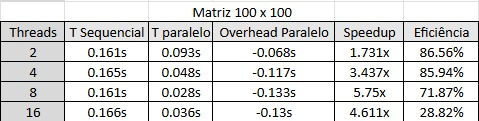
\includegraphics[width=0.7\linewidth]{Strassen100.jpeg}
    \caption{Resultados do paralelismo em matrizes 100x100}
    \label{fig:Strassen100}
\end{figure}
\FloatBarrier

\par A figura 2 abaixo mostra os resultados da multiplicação para uma matriz 200x200. Com uma matriz maior, a perda de eficiência do caso com 16 threads foi inferior ao caso anterior, havendo um pequeno ganho de eficiência em comparação com o caso de 8 threads. Entretanto, apesar do \textit{speedup} superior, a eficiência ainda é baixa, devido ao custo de manutenção de todas as threads.


\begin{figure}[!htbp]
    \centering
    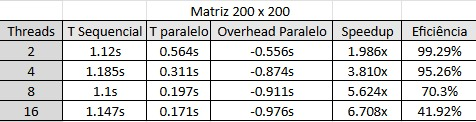
\includegraphics[width=0.7\linewidth]{Strassen200.jpeg}
    \caption{Resultados do paralelismo em matrizes 200x200}
    \label{fig:Strassen200}
\end{figure}
\FloatBarrier


\par Já na figura 3, com uma matriz ainda maior de 300x300, houve novamente um ganho de eficiência para todos os casos, especialmente os casos com 8 e 16 threads. Esse é o resultado esperado e mostra o potencial do paralelismo em casos de multiplicação de matrizes grandes. Apesar da eficiência do caso de 16 threads ainda ser baixa, ele mostrou um \textit{speedup} de mais de 7x, tornando uma execução sequencial de quase 8 segundos em uma execução com paralelismo em pouco mais de 1 segundo.


\begin{figure}[!htbp]
    \centering
    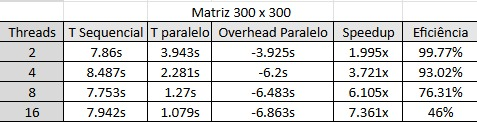
\includegraphics[width=0.7\linewidth]{Strassen300.jpeg}
    \caption{Resultados do paralelismo em matrizes 300x300}
    \label{fig:Strassen300}
\end{figure}
\FloatBarrier


\par Os resultados apresentados mostram, como um todo, que o paralelismo é muito bem aplicado no algoritmo de Strassen, em todos os casos houve um overhead paralelo negativo, mostrando um tempo de execução mais curto para a implementação paralela. Os testes efetuados mostram que o uso de 8 threads gera os resultados mais balanceados entre performance e eficiência, um resultado esperado, visto que o método de Strassen foi paralelizado em suas 7 operações em matrizes independentes.

\section{Conclusão}

\par A implementação e os testes dos algoritmos de multiplicação de matrizes por blocos e de Strassen demonstraram ganhos significativos de desempenho com a execução paralela, intensificados pelo aumento do tamanho das matrizes.
\par Os testes com diversas quantidades de threads do algoritmo de Strassen mostram que, para esse algoritmo, o uso de 8 threads alcança um equilibrio entre speedup e eficiência, obtendo melhorias significativas no tempo de execução, além de seguirem o padrão visto anteriormente de aumento de eficiência baseado no tamanho da matriz. A implementação do paralelismo para as 7 operações de matrizes existentes e a grande eficiência encontrada no uso de 8 threads são resultados encorajadores que mostram o potencial dessas implementações.
\par Os resultados na implementação por blocos demonstram também um forte ganho de eficiência com o uso de paralelismo, com valores de speedup próximos a 8x em algumas instâncias de float e próximo de 9x em algumas instâncias de double. Apesar de alguns problemas de eficiência em casos com blocos pequenos, a estabilização e o ganho de desempenho em blocos maiores mostra o potencial do paralelismo nesse caso também.


\bibliographystyle{sbc}
\bibliography{sbc-template}

\end{document}